%\chapter{GIỚI THIỆU}

\section{Lý do chọn đề tài}

\begin{wrapfigure}{r}[0pt]{0.45\linewidth}
    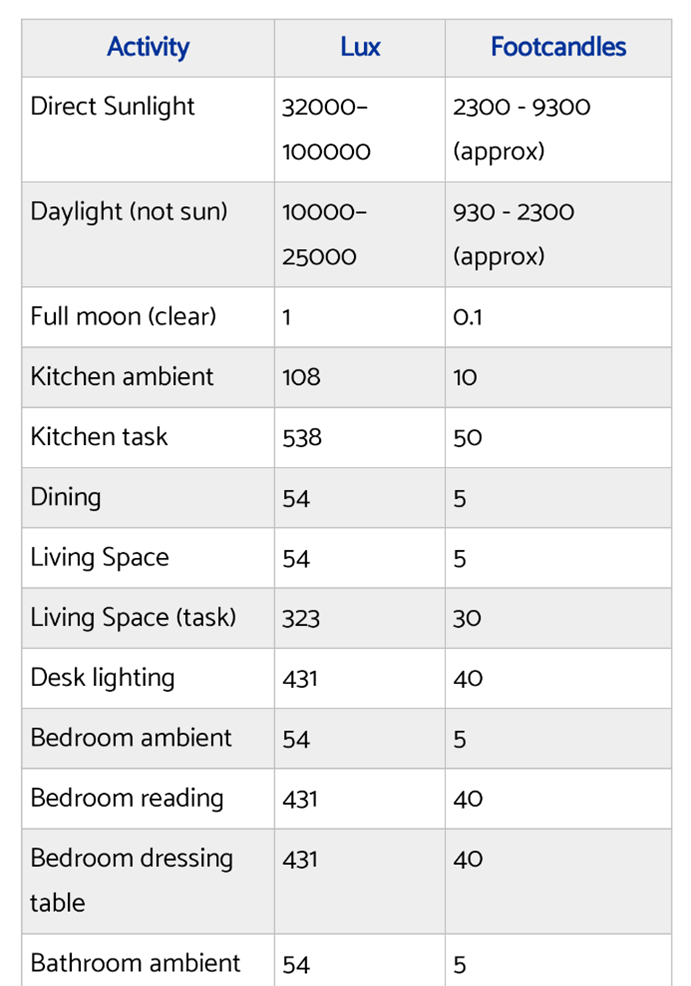
\includegraphics[scale=0.8]{Chapters/Chapter1/Images/Cuongdosangcanthiet}
    \caption{Bảng cường độ ánh sáng cần thiết cho các phòng}
    \label{fig:cuongdoanhsang}
\end{wrapfigure}

Trong hầu hết các hoạt động làm việc, sinh hoạt hằng ngày của con người, luôn cần một lượng ánh sáng nhất định. Tuỳ từng nơi sinh hoạt là phòng khách, phòng ăn (nhà ở) hay là phòng họp, nhà kho (công ty) mà chúng ta sẽ có mức cường độ ánh sáng cần thiết là khác nhau. Có thể thấy trong hình bên, trong nhà bếp, phòng ăn chúng ta chỉ cần 54 lux (đơn vị đo cường độ ánh sáng) còn trong khi đọc sách, chúng ta cần 431 lux. Hiện nay, gần như tất cả các phương án chiếu sáng đều đang sử dụng đèn cố định, tức là không thể thay đổi độ sáng lẫn góc chiếu, vị trí chiếu. Việc này dẫn tới hai nhược điểm sau đây:


Thứ nhất, vào ban ngày khi có ánh sáng tự nhiên, để tránh tình trạng hao phí điện năng thì chúng ta sẽ tắt đèn. Nhưng thường chỉ có những nơi gần cửa sổ, cửa ra vào mới được nhận lượng ánh sáng đầy đủ. Còn ở những nơi xa các nguồn sáng tự nhiên như góc phòng, giữa lớp sẽ có hiện tượng ánh sáng không đủ. Đối với các học sinh sinh viên khi học tập lâu dài trong điều kiện này sẽ dẫn tới các bệnh, tật về mắt.
\begin{center}
    \begin{figure}[ht]
    \begin{center}
     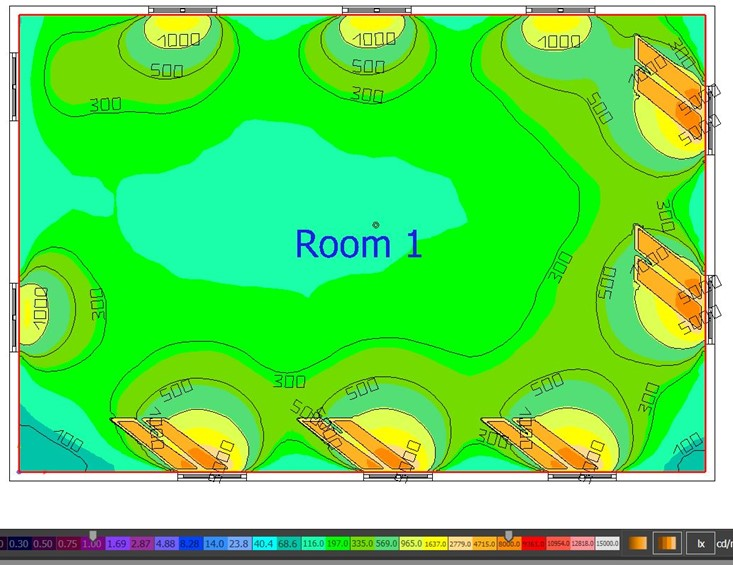
\includegraphics[scale=1]{Chapters/Chapter1/Images/Doroi}
    \end{center}
    \caption{Ảnh hưởng của ánh sáng tự nhiên tới cường độ ánh sáng trong phòng}
    \label{fig:doroi}
    \end{figure}
\end{center}

Thứ hai, thường hệ thống đèn chiếu trong phòng học dùng một vài công tắc để bật tắt toàn bộ đèn trong phòng. Nếu chúng ta bật đèn để khắc phục tình trạng trên thì lại dẫn đến một nhược điểm khác, đó là những nơi có ánh sáng tự nhiên sẽ dư thừa ánh sáng không cần thiết. Khi thiết kế hệ thống chiếu sáng, người thiết kế đã đảm bảo hệ thống đèn sẽ chiếu đủ ánh sáng cần thiết trong điều kiện ban đêm. Khi kết hợp với ánh sáng ban ngày thì sẽ bị dư thừa, gây hao phí điện nặng không cần thiết. Hiện tại, thế giới đang đối mặt với tình trạng nóng lên toàn cầu, việc cắt giảm lượng dư thừa này được áp dụng trên phạm vi rộng chắc chắn sẽ cải thiện một phần nhỏ hiện tượng này. Ngoài ra, việc cắt giảm lượng ánh sáng dư thừa sẽ giúp cho các nhà trường tiết kiệm một khoản tiền điện, điều này có lợi cho ngân sách nhà nước đối với các trường công lập và giảm bớt chi phí phải bỏ ra trong chiếu sáng cho các trường tư, tự chủ.

Do đó, nhóm đã chọn đề tài “ Cân bằng cường độ ánh sáng trong không gian phòng học” với mong muốn có thể cân bằng ánh sáng đều trên cả phòng học, giúp đảm bảo lượng ánh sáng cần thiết trong hoạt động học tập của học sinh, sinh viên và  góp phần tiết kiệm điện năng.

\section{Đối tượng nghiên cứu}
Đối tượng nghiên cứu của đề tài “ Cân bằng cường độ ánh sáng trong không gian phòng học” là: tập trung tìm hiểu, nghiên cứu các vấn đề liên quan, thiết kế và thi công mô hình điều khiển, đưa ra các giải thuật để cân bằng ánh sáng cho không gian trong phòng học.

\section{Mục tiêu nghiên cứu}
\begin{itemize}
\item Đưa ra được các giải thuật cân bằng cường độ ánh sáng trong phòng học.
\item Thực hiện được mô hình phòng học được cân bằng cường độ ánh sáng.
\end{itemize}

\section{Giới hạn đề tài}
Đề tài thực hiện nghiên cứu, thiết kế và thi công mô hình thử nghiệm ở mức độ:
\begin{itemize}
\item Điều khiển cường độ ánh sáng thông qua màn hình máy tính, nút nhấn.
\item Cân bằng bằng cách điều khiển cường độ sáng của đèn hoặc tịnh tiến đèn để đạt được cường độ sáng cần thiết ở mọi điểm trong phòng.
\end{itemize}

\section{Phương pháp nghiên cứu}
Các vấn đề cần nghiên cứu trong đề tài:
\begin{itemize}
\item Phần cứng: Lắp ráp khung mô hình, bộ phận trượt cho dàn đèn, thi công đi dây cho mạch điện, driver điều khiển động cơ step, cảm biến và đèn công suất.
\item Phần mềm: Phần mềm giao tiếp với VĐK từ máy tính bằng giao tiếp UART, chương trình điều khiển hệ thống của VĐK.
\end{itemize}
Phương pháp nghiên cứu:
\begin{itemize}
\item Tìm hiểu tài liệu: tìm hiểu các tài liệu về cường độ sáng, thiết kế chiếu sáng, các phương pháp điều khiển.
\item Tự nghiên cứu: thông qua các tài liệu và các phương tiện thông tin, nhóm tự xây dựng giải thuật, cách xây dựng chương trình.
\item Phương pháp thực nghiệm, thử và thử sai: thực nghiệm điều khiển cân bằng cường độ sáng, qua đó rút ra được kinh nghiệm.
\end{itemize}

\section{Phương pháp thiết kế chung}
\begin{itemize}
\item Sản phẩm: Lập trình điều khiển để cân bằng cường độ ánh sáng trong phòng.
\item Năng suất: Mô hình có thể điều khiển cân bằng ánh sáng với thời gian ngắn và độ chính xác cao.
\item Các thiết kế cơ khí được thiết kế phù hợp với phòng học thực tế.
\end{itemize}





